\documentclass{article}
\usepackage[utf8]{inputenc}
\usepackage[T1]{polski}
\usepackage{classdiagram}


\usepackage[a4paper, margin=1.5cm]{geometry}
\usepackage{tikz}
\usetikzlibrary{calc}

\makeatletter
\def\firstauthor#1{\gdef\@firstauthor{#1}}
\def\@firstauthor{\@latex@warning@no@line{No \noexpand\firstauthor given}}
\def\projectname#1{\gdef\@projectname{#1}}
\def\@projectname{\@latex@warning@no@line{No \noexpand\projectname given}}
\newcommand\makeheader{%

\begin{tikzpicture}
    \node(IN){Imię i nazwisko};
    \node(IN1) at ($(IN) + (0, -0.5)$) {\@firstauthor};
\end{tikzpicture}
\vspace*{20pt}
\begin{center}
    
\begin{tikzpicture}
        \node(PN){\bf\LARGE\@projectname};
        \node(DOK) at ($(PN) + (0, 1)$) {\Large DOKUMENTACJA TECHNICZNA PROJEKTU};
        \node(PDM) at ($(PN) + (0, -1)$) {\Large Przedmiot: PROGRAMOWANIE OBIEKTOWE};
    \end{tikzpicture}
\end{center}
}
\makeatother


\projectname{Warcaby, Java}
\firstauthor{Jan Chlebek}

\begin{document}

\makeheader

\section{Zakres projektu}
 {\small\it Proszę wstawić kilkuzdaniowy opis projektu zawierający informacje:
  \begin{enumerate}
    \item Do czego system będzie wykorzystywany?
          \\
          \textup{Apllikacja jest implementacją gry warcaby. Została stworzona w celach rozrywkowych.}
    \item Jakie są granice używalności tworzonego systemu?
          \\
          \textup{Aplikacja przeznaczona jest do użytku w trybie offline w oknie konsoli, głównie w systemie linux.}
    \item Jaki jest target systemu? (Do kogo system jest skierowany?)
          \\
          \textup{System skierowany jest dla graczy.}
    \item Z czego wynika potrzeba utworzenia systemu?
          \\
          \textup{Projekt zaproponowany wstępnie okazał się zbyt duży. Obecnie posiada kilka tysięcy linii kodu, ponieważ rozwijałem jego koncepcję. Aby oddać skończony projekt przygotowałem tę grę.}
  \end{enumerate}}
\section{Diagram klas}

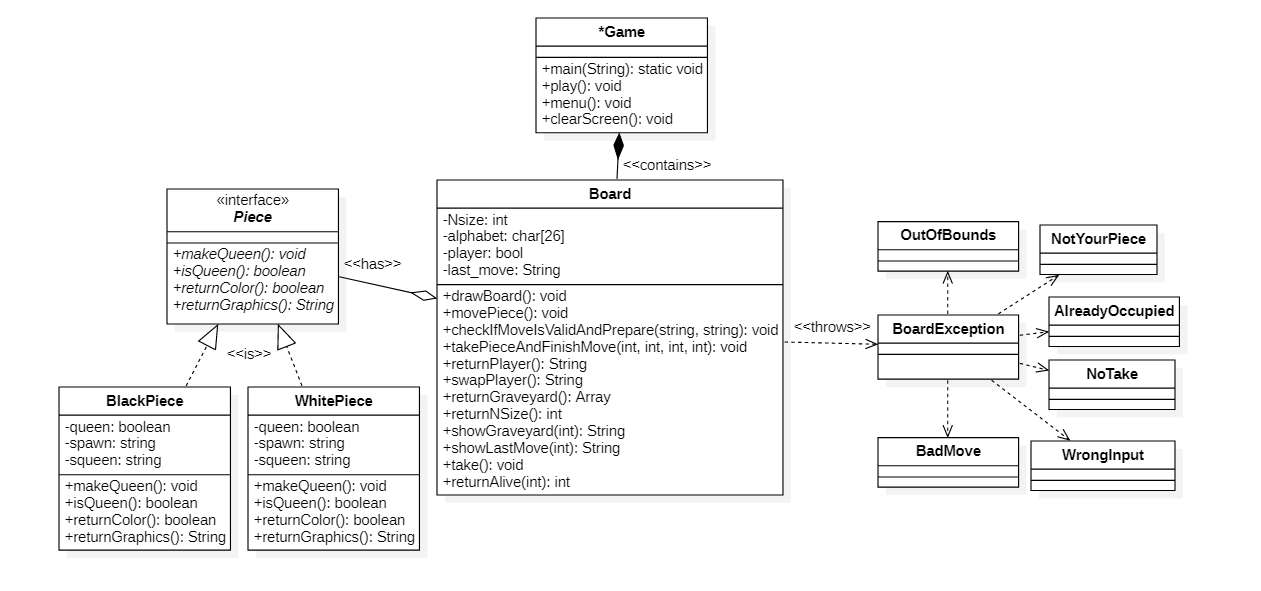
\includegraphics[width=\textwidth]{PO_Java.png}

\section{Wymagania systemowe}
\subsection{Wymagania funkcjonalne}
{\small\it W tym miejscu powinno znaleźć się przynajmniej sześć funkcjonalności do zaimplementowania w projekcie z doperecyzowaniem w podpunktach.}
\begin{enumerate}
  \item Obsługa wyjątków
  \item Wyświetlanie zbitych figur w interfejsie
  \item Widoczny zapis ostatnio wykonanego ruchu
  \item Zabezpieczenia przed niepoprawnie wprowadzonymi danymi wejściowymi
  \item Wbudowana instrukcja obsługi aplikacji
  \item Wyświetlanie dokładnych komunikatów związanych z występującymi wyjątkami
\end{enumerate}
\subsection{Wymagania pozafunkcjonalne}
{\small\it W tym miejscu powinny znaleźć się przynajmniej trzy wymagania pozafunkcjonalne narzucone na aplikację.}
\begin{enumerate}
  \item Wykorzystywanie wyłącznie standardowych bibliotek
  \item Brak odwołań do funkcji systemowych takich jak "cls"
  \item Ograniczenie wykorzystanych znaków do tych obsługiwanych przez większość terminali.
\end{enumerate}
\section{Realizacja projektu}
 {\small\it W tym miejscu proszę opisać procedurę, zgodnie z którą projekt będzie realizowany, np. jaka jest koncepcja zbioru bibliotek do wykorzystania przez system (ewentualnie kryteria zgodnie z którymi biblioteki będą wybierane), jakie jest wyobrażenie rytmu pracy nad projektem, jaki jest ramowy plan realizacji z wyszczególnieniem kroków milowych do celu utworzenia systemu.}
\\ \\
\textup{Projekt zrealizowany został w dwóch sprintach skupiających się na implementowaniu klas zgodnie z diagramem UML rozpoczynając od tych najbardziej zewnętrznych.  Ramowy plan zakłada najpierw realizację podstawowych funkcjonajlności niezbędnych do inicjalizacji sztabu, następnie przygotowania systemu rozliczeń i baz danych. Projekt został zrealizowany jako substytut (celem zaliczenia przedmiotu) niedokończonego i nieopublikowanego projektu, który ciągle realizuję.}
\section{Kryteria akceptacyjne}
\begin{enumerate}
  \item Rozpoczęcie gry poprzez uruchomienie aplikacji w systemie linux (main znajduje się w pliku Game.java)
  \item Przeczytanie instrukcji i wpisanie "start" celem przetestowania rozgrywki
  \item Testy odporności
  \item Audyt kodu
\end{enumerate}
\end{document}

